\chapter{Máquinas de aprendizaje}
\label{ch:chapter1}
 
El Aprendizaje de Máquina toma como base dos áreas de investigación:
la Ciencia de la Computación y la Estadística. De la primera, retoma las preguntas: ¿Cómo se pueden construir máquinas que resuelvan problemas? Y ¿Qué problemas son tratables o intratables? De la segunda, toma las preguntas: ¿Qué puede ser inferido de los datos? ¿Bajo que supuestos del modelo? Y ¿Con qué confiabilidad? \cite{mitchell2006discipline}. El esfuerzo por resolver estas preguntas da como resultado una disciplina enfocada a construir teorías estadístico-computacional de los procesos de aprendizaje.

\section{Procesos de aprendizaje}

Se dice que una máquina ``aprende" dada una tarea (T), una medición del rendimiento (R) y un tipo de experiencia (E) si el sistema mejora confiablemente su rendimiento (R) en la tarea (T) dada la experiencia (E) \cite{mitchell2006discipline}. Es decir, se modela una estructura con los datos proporcionados de manera que el rendimiento en la tarea mejora conforme más información recibe. La diversidad de las tareas, así como el campo de aplicaciones es muy diverso, por ejemplo:

\begin{itemize} 

\item \textit{Clasificación de spam/no-spam}, en el que (E) son los correos, (T) el clasificar correctamente el \textit{spam} y (R) el porcentaje de correos correctamente clasificados.

\item \textit{Reconocimiento/Clasificación facial}, en el que (E) son los rostros de distintas personas, (T) el reconocimiento o clasificación de los rostros y (R) el porcentaje de rostros correctamente reconocidos o clasificados.

\end{itemize} 

Los procesos de aprendizaje tienen diversas aplicaciones y distintos supuestos, por lo que han surgido clasificaciones para analizarlos en conjunto. La clasificación que se tomó en este texto es la propuesta por T. Hastie \cite{hastie2009elements}, la cual divide a los métodos en dos grupos: aprendizaje supervisado y aprendizaje no supervisado. El primero, supone la presencia de una variable de salida que actúa como guía en la construcción de la estructura. Ejemplos de éste es la regresión lineal, los árboles de decisión y las máquinas de soporte vectorial. Por otra parte, el aprendizaje no supervisado solo cuenta con la información de las variables independientes; por ejemplo, análisis de conglomerados, reglas de asociación y algunos métodos de reducción dimensional. 

Después de esta primera clasificación, se subclasifica a los métodos de aprendizaje supervisado de acuerdo al tipo de variable de salida (Figura 1.1). \footnote{A lo largo del texto se usará indiferentemente variable de entrada como ``input'' o variable independiente y variable de salida como ``output'' o variable dependiente} Cuando se trata de una variable cuantitativa recibe el nombre de regresión, mientras que en el caso de cualitativas se le llama clasificación. Por otra parte, el aprendizaje no supervisado tiene dos ramas en las que el texto hace énfasis \cite{hastie2009elements}. Segmentación en el caso que se desee asignar un grupo a cada individuo, de manera que los grupos sean homogéneos entre sí; o bien, reducción dimensional cuando solamente se desea proyectar a los individuos en un espacio de menor dimensión, de manera que se cumplan características especiales en dicho subespacio. 

En esta tesis se tratarán principalmente problemas de aprendizaje supervisado, haciendo especial énfasis a problemas de clasificación. Al ver el problema a tratar se elige un método para resolverlo; por ejemplo, para problemas de clasificación se utiliza comúnmente la Regresión Logística, el Análisis Discriminante Lineal y las Máquinas de Soporte Vectorial. En cambio, para problemas de regresión son comúnmente usados las regresiones lineales y no lineales. También hay otros métodos que sirven para ambas finalidades, como lo son los bosques aleatorios. 

\begin{figure}[!ht]
  \centering
	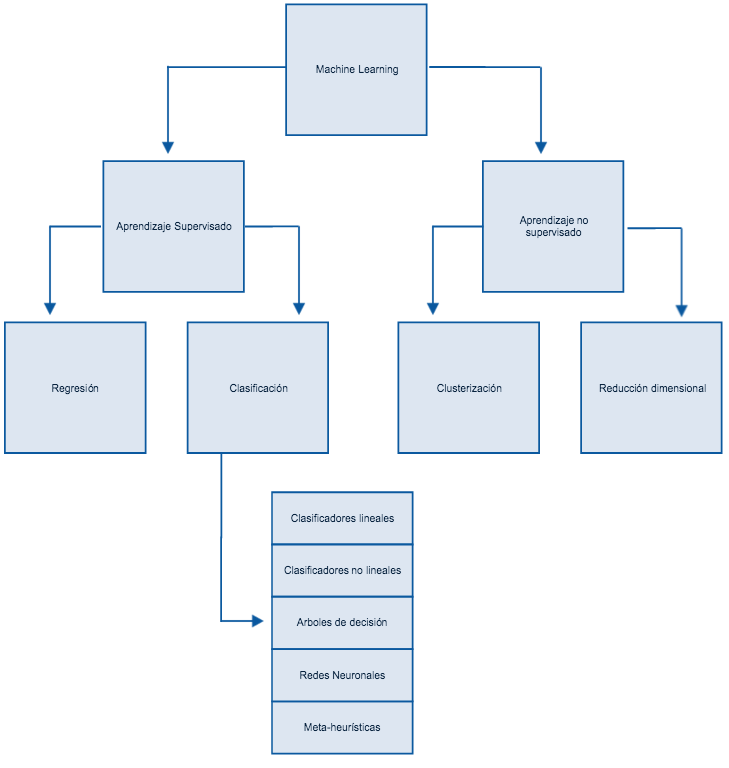
\includegraphics[width=1\textwidth]{Figures/Chapter1_Clasificacion}	
  \caption[Enfoques para resolver problemas de clasificación]
  {Distintos enfoques para resolver problemas de clasificación en el área de Aprendizaje de Máquina.}
\end{figure}

\subsection{Fase de inferencia y fase de decisión}

Como primer paso, una vez elegido el método, se selecciona el criterio de penalización de los errores. Este debe ser elegido de manera acorde al problema planteado; por ejemplo, en el caso de una regresión lineal se desea que la penalización sea mayor en los datos que queden muy lejos del ajuste lineal, por lo que se escoge la norma euclidiana \footnote{Además de que las estimaciones hechas a través de mínimos cuadrados bajo ciertos supuestos tienen propiedades deseables de los estimadores: Que sean insesgados y de varianza mínima} $||x||_2 = \sqrt[]{x_{1}^{2}+x_{2}^{2}+ ... + x_{n}^{2}}$. En cambio, en un problema de clasificación se escoge una matriz de penalización o matriz de pérdida, en la que se establece el costo por cada tipo de error de clasificación.

Como segundo paso, se procede con la fase de inferencia, en la que se ajustan los estimadores de los parámetros del modelo elegido de acuerdo a los datos que se tienen, esto con el fin de hacer la inferencia de las distribuciones poblacionales. Como tercer y último paso, se procede a la fase de decisión, en la que se busca encontrar un criterio de decisión que minimice la pérdida esperada \cite{bishop2006pattern}. Por ejemplo, para los problemas de clasificación es muy claro determinar estas dos fases: la primera, se lleva a cabo al determinar la distribución conjunta de clases de pertenencia e individuos; mientras que la segunda, se realiza al determinar las fronteras de decisión basadas en estas probabilidades. Por otra parte, para los problemas de regresión tradicional, ambas fases se realizan al mismo tiempo, ya que al calcular los estimadores de los parámetros se utiliza el método de mínimos cuadrados que minimiza la penalización cuadrática.


\section{Clasificación con modelos lineales}


Se comenzará definiendo la nomenclatura utilizada en esta tesis. Las clases se denotan con la variable aleatoria $k \in C$, con $C  = \{ k = k_j: j = 1, \vdots, K\}$ el conjunto de posibles clases a clasificar y $n(C) = K$ la cardinalidad del conjunto. Para los individuos se define la variable aleatoria $x \in {\rm I\!R}^{m}$. De esta manera, sea $p(x, k)$ \footnote{Teniendo esta probabilidad se pueden calcular fácilmente las probabilidades condicionales $p(k|x)$ y $p(x|k)$} la distribución conjunta de individuos $x$ con clases $k$.


Para la fase de inferencia se utilizan los datos de entrenamiento, donde se distingue a los individuos y a sus clases de pertenencia $x_i \in  {\rm I\!R}^{m}$ y $y_i \in {\rm I\!R}$ respectivamente, con $i = 1, ... , N$. Agrupándolos en matrices, sea $X \in {\rm I\!R}^{N \times m}$ la matriz de individuos y $Y \in {\rm I\!R}^{N \times 1}$ el vector de clases de pertenencia asociada a cada individuo. Una vez hecha la inferencia, se pueden encontrar clases predichas para los individuos $x_i$, se denotará como $\widehat{y_i}$ y $\widehat{Y}$ a la respectiva matriz.


\begin{table}
\caption{Nomenclatura usada en el texto}
\begin{center}
    \begin{tabular}{ | l | c | c | p{4.5cm} |}
    \hline
    Tipo & Definición & Valores & Descripción  \\ \hline
    Entero & $K$ & $K \in \mathbb{N}$ & Número de posibles clases. \\ \hline
    Entero & $N$ & $N \in \mathbb{N}$ & Número de individuos en los datos. \\ \hline
    Entero & $N_k$ & $N_k \in \mathbb{N}$ & Número de individuos en la clase $k$. \\ \hline
    Entero & $m$ & $m \in \mathbb{N}$ & Dimensión de los individuos. \\ \hline
    v.a. & $k$ & $k \in C$ & Variable aleatoria de las clases. \\ \hline
	v.a. & $x$ & $K \in {\rm I\!R}^{m}$ & Variable aleatoria de los individuos. \\ \hline
    Conjunto & $C$ & $k_j: j = 1 ... K$ & Conjunto de posibles clases. \\ \hline
    Dato & $x_i$ & $x_i: i = 1 ... N$ & Vector columna del individuo $i$. \\ \hline
    Dato & $y_i$ & $y_i: i = 1 ... N$ & Dato de clase real del individuo $i$. \\ \hline
    Dato & $\widehat{y_i}$ & $\widehat{y_i}: i = 1 ... N$ & Dato de clase predicha del individuo $i$. \\ \hline
    Dato & $X$ & $X^T = [x_1 |...| x_N]$ & Matriz de individuos. \\ \hline
    Dato & $Y$ & $Y^T = [y_1 | ... | y_n]$ & Vector de clases reales de infividuos. \\ \hline
    Datos & $\widehat{Y}$ & $\widehat{Y}^T = [\widehat{y_1} | ... | \widehat{y_n}]$ & Vector de clases predichas de infividuos. \\ \hline
    Distribución & $p(x,k) $ &  & Distribución conjunta de individuos y clases \\ \hline
    \end{tabular}
\end{center}
\end{table}


\subsection{Fase de inferencia}
Como se mencionaba antes, en fase de inferencia se busca encontrar la distribución conjunta de la muestra con cada una de las clases, es decir $p(x,k)$. La dificultad en estimar esta distribución aumenta conforme la dimensionalidad de $x$ crece y conforme el número de clases aumenta \footnote{Para poder estimar la distribución conjunta, el número de clases debe ser menor que el conjunto de individuos}. Esto es debido a que se comienza a requerir un conjunto de datos mayor para poder estimar cada punto de $p(x,k)$. Por esta razón, muchas veces es suficiente encontrar directamente $p(k|x)$; es decir, dadas las características del individuo, encontrar que tan probable es que pertenezca a cada clase. Por otro lado, en la fase de decisión se encuentra la asignación óptima dependiendo de la matriz de pérdida que se seleccionó y de las probabilidades calculadas (ya sea la distribución conjunta o las condicionales). 

Los modelos propuestos para resolver la fase de inferencia se pueden agrupar de la siguiente manera \cite{bishop2006pattern}: 

\begin{enumerate}
	\item  \textbf{Modelos Probabilísticos Generativos.}
    Plantean resolver el problema de inferencia con el objetivo de determinar $p(x,k)$; es decir, la distribución conjunta de individuos y clases. Una vez obtenida la distribución, se puede usar para calcular $p(x|k)$, $p(k|x)$, $p(x)$ o $p(k)$. Para este enfoque se tienen que hacer supuestos acerca de la distribución de $x$ o $x|k$, o bien, tener un conjunto de entrenamiento muy grande que permita inferir acertadamente $p(x,k)$.

    Tomando propiedades básicas de probabilidad, se pueden calcular las distribuciones necesarias:
  
    \begin{equation} \label{eq:1}
     p(x, k) = p(x|k) p(k)
    \end{equation}

    \begin{equation} \label{eq:2}
     p(x, k) = p(k|x) p(x) 
    \end{equation}
    
    \begin{equation} \label{eq:3}
     p(k|x)  = \frac{p(x|k)p(k)}{p(x)}
    \end{equation}

	\begin{equation} \label{eq:4}
	 p(x) = \sum_{k} p(x|k)p(k) 
	\end{equation}
	
	\begin{equation} \label{eq:5}
	 p(k) = \sum_{x} p(k|x)p(x) 
	\end{equation}
	
	En caso de no tener suficientes datos para inferir directamente esta distribución; o bien, de no tener conocimiento de la estructura de la distribución de $x$, se dan preferencia a los modelos discriminativos o modelos de funciones discriminantes.

\textit{Ventajas\cite{bishop2006pattern}:}
\begin{itemize}
\item Puede ser útil para detectar datos atípicos, ya que al supone una distribución de $x$, se puede determinar qué puntos son poco probables de suceder. De esta manera, se puede encontrar qué predicciones podrían fallar. 
\end{itemize}

\textit{Desventajas\cite{bishop2006pattern}:}
\begin{itemize}
\item Se debe tener información acerca de la distribución de $x$.

\item Inferir directamente de los datos la distribución $p(x,k)$ puede ser muy demandante cuando la dimensionalidad de $x$ es alta. 

\item Si solo se requiere hacer clasificación, puede ser ineficiente encontrar toda la distribución conjunta.
\end{itemize}


\item \textbf{Modelos Probabilísticos Discriminativos.}
Primero, se resuelve el problema de inferencia para determinar $p(k|x)$ con los datos, y después se procede a la fase de decisión para asignar la clase de pertenencia.

\textit{Ventajas:\cite{bishop2006pattern}}
\begin{itemize}
\item Solo se necesita estimar $p(k|x)$ y no toda la distribución conjunta.
\end{itemize}

\textit{Desventajas:\cite{bishop2006pattern}}
\begin{itemize}
\item No se tiene la detección de atípicos presentados por el primer enfoque.
\end{itemize}


\item \textbf{Función Discriminante}
Plantea encontrar una función $\widehat{f}:{\rm I\!R}^m \rightarrow {\rm I\!R}$, tal que clasifique directamente a cada individuo en una clase $k$, de esta manera se define $\widehat{Y}=\widehat{f}(x)$. 

\textit{Ventajas:\cite{bishop2006pattern}}
\begin{itemize}
\item Se combina la fase de inferencia y la fase de decisión en una sola función $\widehat{Y}=\widehat{f}(x)$. 
\end{itemize}

\textit{Desventajas:\cite{bishop2006pattern}}
\begin{itemize}
\item Ya no se cuenta con las probabilidades posteriores $p(k|x)$, por lo que ya no se puede analizar una a una la probabilidad de pertenencia del individuo $x$ a cada una de las clases.
\end{itemize}

\end{enumerate}


\subsection{Fase de decisión}
Para la fase de decisión es conveniente analizar tres definiciones: ``Regiones de decisión'',  ``Fronteras de decisión'' y  ``Funciones discriminantes''. Las primeras dos reciben este nombre porque buscan dividir el espacio al que pertenecen los datos en regiones distintas y excluyentes. Cada una de estas regiones $R_{k}$ clasifica al individuo $x$ en una única clase $k$. En cambio, las fronteras de decisión son las zonas que delimitan una región de las demás; es decir, en ellas (o en sus cercanías) es indiferente qué clase elegir. Por esta razón, es conveniente analizar los datos que quedan cercanos para poder hacer una elección, tomando en cuenta la naturaleza del problema. Por último, las Funciones Discriminantes, nos permiten comparar directamente qué tan verosímil es que un individuo pertenezca a una clase u a otra.

Debido a la finalidad del texto se proponen fronteras lineales \footnote{Las fronteras de decisión pueden tomar formas irregulares, pero en general su forma depende del método de clasificación elegido}, ya que al igual que una regresión lineal, es la base que ejemplifica modelos más complejos. Por este motivo, se mostrarán distintas opciones para construir las regiones y fronteras que se adecuan a los tres enfoques distintos: modelos probabilísticos generativos, modelos probabilísticos discriminativos y funciones discriminantes. 

Para asegurar la linealidad en las fronteras, se debe hacer un análisis que garantice esta propiedad. Se ejemplificará con un caso de dos clases: $k_i$ y $k_j$ con $\left( \begin{array}{ccc}
0 & c_{ij} \\
c_{ji} & 0 \\
 \end{array} \right)$, la matriz de costos con $c_{ij}$ el costo de elegir $i$ cuando la verdadera clase es $j$. Se supone que $c_{ij}, c_{ji}$ mayores que 0. De esta manera la frontera de decisión está dada por:

\begin{equation} \label{eq:6}
c_{ij} p( k = k_i | x \in k_j) - c_{ji} p(k = k_j| x \in k_i) = 0
\end{equation}

De otra manera, si $c_{ij} p( k = k_i | x \in k_j) < c_{ji} p( k = k_j| x \in k_i) $ o viceversa, entonces se clasificará hacia $k_i$ y $k_j$, respectivamente. Para los fines de esta tesis, se tomarán los costos de $c_{ij} = c_{ji} = 1$ ya que esto solo juega en la ordenada al origen de la ecuación de la frontera lineal. Tomando un resultado presentado por T. Mitchell \cite{mitchell2006discipline}, si se aplica una función monótona de $p(k, x)$, la linealidad de las fronteras de decisión se mantiene. En este caso, se toma la función de logaritmo $log()$:


$$ log(p(k = k_j | x)) = log( p(k = k_i | x)) $$	

\begin{equation} \label{eq:7}
 log \frac{p( k = k_j | x )}{ p(k =  k_i |  x)} = 0 	
\end{equation}

El lado izquierdo de esta última ecuación es conocido como razón de momios (log odd). Cuando es una función lineal con respecto a $x$, mantiene la linealidad de la frontera:

\begin{equation} \label{eq:8}
 log \frac{p(k = k_j | x )}{p(k = k_i |  x)} = \beta_0 + x^T \beta_1 
\end{equation}


\section{Métodos de clasificación lineales}

En la fase de inferencia se busca construir la distribución $p(x,k)$, la cual será usada en la fase de decisión para tomar un criterio óptimo de clasificación. En la sección 2.2 se mostraron los distintos enfoques que se toman para hacer esta inferencia. Recapitulando, para modelos generativos se escoge $\widehat{Y}(x) = \widehat{f}(p(x,k))$; para modelos discriminativos $\widehat{Y}(x) = \widehat{f}(p(k|x))$ y para funciones discriminantes se escoge $\widehat{Y}(x)$ = $\widehat{f}(x)$. En los dos primeros casos se ve que la función $f$ toma como entrada distribuciones concernientes a $x$ y $k$, pero en el tercer caso, solamente toma como entrada a $x$. En esta sección se ejemplificarán los 3 métodos con técnicas sencillas. Para el enfoque Probabilístico Generativo se empleará el Análisis Discriminante Lineal, para el Probabilístico Discriminativo la Regresión Logística y para la función discriminante, el Discriminante Lineal de Fisher.

En los siguientes tres ejemplos se explica cómo se realiza la inferencia de las distribuciones, para después demostrar la linealidad en las fronteras. Como se explica en la sección 2.2.2, si se asegura que (\ref{eq:8}) es lineal con respecto a $x$, entonces se garantiza la linealidad de estas. En la Regresión Logística se ejemplificará el procedimiento para $n$ clases. Para los demás se supondrá el caso de la frontera entre dos clases.


\subsection{Modelos discriminativos: Regresión Logística}


\textit{Inferencia de la distribución $p(k | x)$} \\
Para la fase de inferencia, se calculan las probabilidades posteriores de pertenecer a cada grupo $j$, de manera que: 
\begin{equation} \label{eq:15}
	\sum\limits_{j = 1}^{K} p(k = k_j | x) = 1
\end{equation}


\textit{Linealidad de la frontera}\\
Para obtener la estimación de las $K$ distribuciones de probabilidad $p(k = k_j | x)$, se parte de la ecuación (\ref{eq:8}) y se supone que todas las fronteras son lineales.

$$ \log \frac{p(k = k_1 | x)}{p(k = k_K | x)} = \beta_{1.0} + \beta_1^T x$$

$$ \log \frac{p(k = k_2 | x)}{p(k = k_K | x)} = \beta_{2.0} + \beta_2^T x$$

$$\vdots$$

$$ \log \frac{p(k = K-1 | x)}{p(k = k_K | x)} = \beta_{(K-1).0} + \beta_{(K-1)}^T x$$

Con estas ecuaciones se crea un sistema que cuenta con $K$ variables $p(k = k_j| x)$ y $K-1$ ecuaciones, lo cual, añadiendo la restricción (\ref{eq:15}) se puede despejar cada probabilidad: 

$$ p(k = k_1 | X = x) = \frac{\exp(\beta_{1.0} + \beta_1^T x)}{1+\sum\limits_{i=1}^{K-1} {\exp(\beta_{l.0} + \beta_l^T x)}} $$

$$ p(k = k_2 | X = x) = \frac{\exp(\beta_{2.0} + \beta_2^T x)}{1+\sum\limits_{i=1}^{K-1} {\exp(\beta_{l.0} + \beta_l^T x)}} $$

$$ \vdots $$

$$ p(k = k_{K-1} | X = x) = \frac{\exp(\beta_{(K-1).0} + \beta_{(K-1)}^T x)}{1+\sum\limits_{i=1}^{K-1} {\exp(\beta_{l.0} + \beta_l^T x)}} $$

Para la clase de referencia: 

$$ p(Y = k_K | X = x) = \frac{1}{1+\sum\limits_{i=1}^{K-1} {\exp(\beta_{l.0} + \beta_l^T x)}} $$

Para tener la formulación completa, falta estimar las $\beta$ de cada probabilidad. Esto, comúnmente, se realiza con máxima verosimilitud (a través de métodos iterativos como Newton) \cite{hastie2009elements}


\textit{Funciones $logit$ y $logit^{-1}$} \\
Para este modelo es conveniente analizar la función logit y su inversa:
 
 \begin{equation} \label{eq:16}
 logit = \log (\frac{p}{1-p}) 
 \end{equation}

\begin{equation} \label{eq:17}
 logit^{-1}  = \frac{\exp(x)}{1+\exp(x)}
 \end{equation}


Al graficar la función $logit$ y la $logit^{-1}$ sobre un plano (Figura 1.1) se observan algunas de sus propiedades. En la gráfica de la izquierda, se realiza un mapeo de valores del rango (0,1) al rango (-$\inf$,$\inf$), mientras que a la derecha se transforman valores continuos de (-$\inf$, $\inf$) al $(0,1)$. La transformación realizada por $logit^{-1}$ es de mayor interés ya que su rango es semejante al que toman las probabilidades. Este enfoque nos da una amplia gama de elección para la fase de decisión, ya que deja elegir los puntos de corte para cada clase, dependiendo la penalización que se quiera dar a cada tipo de error \cite{hastie2009elements}:

\begin{figure}[!ht]
  \centering
	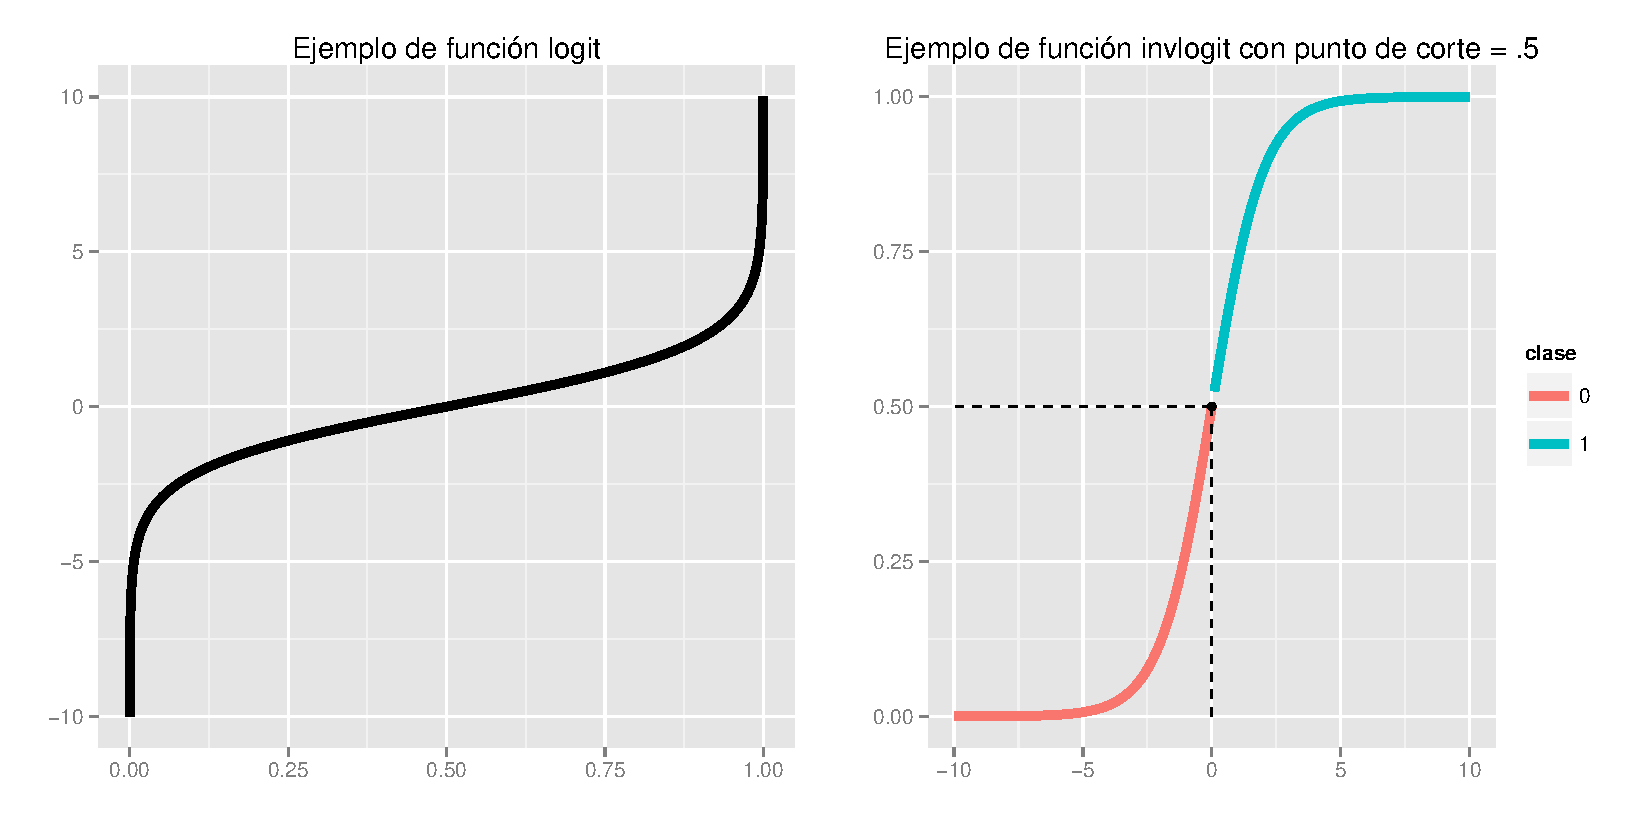
\includegraphics[width=1\textwidth]{Figures/Chapter1_logit}	
  \caption[Función logit y $logit^{-1}$]
  {En la izquierda se muestra la función logit y en la derecha la función $logit^{-1}$ con punto de corte p = .5; es decir, se escoge la clase 1 en la zona azul y la clase 0 en la zona roja.}
\end{figure}

\pagebreak
\subsection{Modelos generativos: Análisis Discriminante Lineal}


\textit{Inferencia de la distribución $p(x,k)$}\\
Para el caso del Análisis Discriminante Lineal se sigue un enfoque generativo, en el que se realiza inferencia de $p(x,k)$. Primero, se supondrá que $p(x|k)$ sigue una distribución Gaussiana con varianza $\Sigma_{k}$ constante para todas las clases y $\mu_{k}$ la media de los individuos pertenecientes a la clase $k$ (ecuación (\ref{eq:9})). Por otra parte, se estima la distribución $p(k)$ como la proporción de casos que cada clase aparece en los datos (ecuación (\ref{eq:10})). Usando la ecuación (\ref{eq:1}) se deduce $p(x,k)$:


\begin{equation} \label{eq:9}
 p(x|k) = \frac{1}{(2\pi) |\Sigma|^{1/2}} e^{-\frac{1}{2}(x-\mu_{k})^{T}\Sigma^{-1}(x-\mu_{k})}
\end{equation}

\begin{equation} \label{eq:10}
 p(k) = \frac{N_k}{N}	
\end{equation}

Por otro lado, al utilizar el Teorema de Bayes (\ref{eq:3}) y la ecuación (\ref{eq:4}), se puede calcular $p(k|x)$ directamente. 



\textit{Linealidad de la frontera}\\
Al hablar de la linealidad de la frontera, se tiene que cumplir la ecuación (\ref{eq:8}), enunciada en la sección 2.2.2:

$$\log \frac{p(k = k_j | x )}{p(k = k_i |  x)} = \beta_0 +  x^T \beta_1$$

$$\log \frac{p(x | k = k_j)p(k = k_j)}{p( x | k = k_i)p(k = k_i)} = \beta_0 +  x^T \beta_1$$

\begin{equation} \label{eq:11}
 	\log\frac{p(x | k = k_j)}{p(x | k = k_i)} + \log\frac{p(k = k_j)}{p(k = k_i)} = \beta_0 +  x^T \beta_1
\end{equation} 

La ecuación (\ref{eq:11}) consta de dos sumandos. Al desarrollar el primero:

$$ \log\frac{p(x | k = k_j)}{p(x | k = k_i)} = -\frac{1}{2}[(x - \mu_j)^T \Sigma^{-1}(x - \mu_j) - (x - \mu_i)^T \Sigma^{-1}(x - \mu_i)] $$ 


\begin{equation}
\begin{aligned}
 \log\frac{p(x | k = k_j)}{p(x | k = k_i)} =& -\frac{1}{2}[{\mu_j}^T \Sigma^{-1} {\mu_j}  -  {\mu_i}^T \Sigma^{-1} {\mu_i}]  + \\
 &\frac{1}{2}[{x}^T \Sigma^{-1}(\mu_j-\mu_i) - {(\mu_j-\mu_i)}^T \Sigma^{-1}(x)
\end{aligned}
\end{equation}

 

 \begin{equation} \label{eq:12}
 	\log\frac{p(x| k = k_j)}{p(x | k = k_i)} = -\frac{1}{2}[{(\mu_j - \mu_i)}^T \Sigma^{-1} {(\mu_j + \mu_i)}] + [{x}^T \Sigma^{-1}(\mu_j-\mu_i)]
 \end{equation}

Sustituyendo \ref{eq:12} en \ref{eq:11} se tiene como resultado:

$$ \log \frac{p(k = k_j)}{p(k = k_i)} - \frac{1}{2}[(\mu_j - \mu_i)^T \Sigma^{-1} (\mu_j + \mu_i)] + {x}^T \Sigma^{-1} (\mu_j - \mu_i) = \beta_0 +  x^T \beta_1$$

Del cual se nota que $\beta_0$ y $\beta_1$ son equivalentes a:

\begin{equation} \label{eq:13}
\beta_0 = \log \frac{p(k = k_j)}{p(k = k_i)} - \frac{1}{2}[(\mu_j - \mu_i)^T \Sigma^{-1} (\mu_j +\mu_i)] 	
\end{equation}

\begin{equation} \label{eq:14}
 \beta_1 = \Sigma^{-1} (\mu_j -\mu_i)
\end{equation}


\textit{Funciones Discriminantes} \\
Ahora, solo falta enunciar las funciones discriminantes de la clase $i$ y $j$; es decir, $log p(k = k_i | x)$ y  $log p(k = k_j | x)$, respectivamente:
$$ \delta_j (x) = \log {p(k = k_j)} - \frac{1}{2}\mu_j^T \Sigma \mu_j + x^T \Sigma^{-1} \mu_j$$
$$ \delta_i (x) = \log {p(k= k_i)} - \frac{1}{2}\mu_i^T \Sigma \mu_i + x^T \Sigma^{-1} \mu_i$$


\subsection{Funciones Discriminantes: Discriminante Lineal de Fisher}

El Discriminante Lineal de Fisher es similar al Análisis Discriminante Lineal. El primero permite ver una proyección informativa en un espacio de dimensión menor \cite{hastie2009elements}. Este planteamiento fue propuesto por Fisher \cite{fisher1936use}, y hace referencia a un discriminante lineal con menos supuestos \footnote{No toma en cuenta la distribución de los datos, ni la igualdad de varianzas entre las clases.}. Propone los supuestos de definir una varianza entre clases que es la varianza de las medias de las clases, y una varianza intra-clase, que mide la varianza dentro de las clases con respecto a la media de cada clase. Después, se busca una matriz de proyección $V$ que maximice la dispersión entre-clase al mismo tiempo que minimiza la dispersión intra-clase \cite{ngo2012trace}.

Se comenzará definiendo la nomenclatura necesaria para la sección. Sea $N_{k}$ el número de personas en la clase $k$, $N$ el número total de personas y $w_i = V^T x_i$; es decir, los datos proyectados con la matriz $V$. Entonces, se definen las medias de grupo $k$ como $\mu_k$ y la media de todos los datos $x_i$ como $\mu$:

\begin{equation} \label{eq:18}
 	\mu_k = \frac{1}{N_{k}} 
 	\sum_{\substack{i = 1\\
                  	y_i = k}}^{N}
                  x_i
\end{equation} 


\begin{equation} \label{eq:19}
 \mu = \frac{1}{N} \sum_{i = 1}^{N} x_i
\end{equation}

Por otro lado, se definen las medias correspondientes a los datos proyectados $w_i$:
\begin{equation} \label{eq:20}
 	\widetilde{\mu_k} = \frac{1}{N_{k}} 
 	\sum_{\substack{i = 1\\
                  	y_i = k}}^{N}
                  w_i
\end{equation} 


\begin{equation} \label{eq:21}
 \widetilde{\mu} = \frac{1}{N} \sum_{i = 1}^{N} w_i
\end{equation}


La matriz de dispersión intra-clase de los datos proyectados:


$$\Phi_{I} = \sum_{k=1}^{K} 
				\sum_{\substack{i = 1\\
                  			   	y_i = k}}
                    ^{N}
           ||w_i-\widetilde{\mu}_{k}||^{2}_{2}$$


$$ \Phi_{I} =  \sum_{k=1}^{K} 
					\sum_{\substack{i = 1\\
                  			   	y_i = k}}
                    ^{N}
			Tr (V^T (x_i - \mu_k)(x_i - \mu_k)^T V ) $$

\begin{equation} \label{eq:22}
 \Phi_{I} =  Tr(V^T S_I V) 
\end{equation}



\begin{equation} \label{eq:23}
con \quad S_I = \sum_{k=1}^{K} 
					\sum_{\substack{i = 1\\
                  			   	y_i = k}}
                    ^{N}
 ({x_i-\mu_{k}})({x_i-\mu_{k}})^T 
\end{equation}



La matriz de dispersión entre-clases de los datos proyectados:

$$ \Phi_{E} = \sum_{k=1}^{K} N_{k} || \widetilde{\mu}_k - \widetilde{\mu} ||^{2}_{2} $$

$$ \Phi_{E} = \sum_{k=1}^{K} N_{k} || V^T \mu_k - V^T \mu ||^{2}_{2} $$
 
$$ \Phi_{E} =  \sum_{k=1}^{K} N_{k} V^T(\mu_k - \mu)(\mu_k - \mu)^T V $$
\begin{equation} \label{eq:24}
 \Phi_{E} =  Tr(V^T S_E V)  
\end{equation}

\begin{equation} \label{eq:25}
 con \quad S_E = \sum_{k=1}^{K} N_{k} (\mu_k - \mu)(\mu_k - \mu)^T 
\end{equation}

De este modo, se definen las dos matrices importantes del método: $S_I$ la matriz de dispersión interna y $S_E$ la matriz de dispersión entre clases. Con estas definiciones surge la idea intuitiva de maximizar $\Phi_{E}$ al mismo tiempo que se minimiza $\Phi_{I}$; es decir, encontrar un espacio de proyección en el que los grupos pertenecientes a la misma clase tengan poca varianza, al mismo tiempo que la varianza entre estas clases sea alta. Se puede plantear esta idea a través del problema de maximización:

\begin{equation}\label{eq:26}
	\max_{\substack{V \in {\rm I\!R}^{n\times p} \\ V^TV = I}} \frac{Tr(V^T S_E V)}{Tr(V^T S_I V)} 
\end{equation}

Este problema de optimización es el principal tema de la tesis, por lo que los detalles acerca de las fronteras y el proceso de maximización que derivan en encontrar la matriz óptima $V$ será analizado en los capítulos siguientes.

\section{Enfoques para la minimización del error}

La teoría de la decisión se aplica para la fase dos, en la que se busca tomar decisiones óptimas dadas las probabilidades calculadas en la fase de inferencia. La motivación de una teoría de la decisión es que las probabilidades, por sí solas, no nos indican que clase elegir, solamente nos dan información del comportamiento de la distribución. Por esta razón, es conveniente saber que decisión tomar basándonos en la penalización de los errores elegidos anteriormente. Puede verse desde dos perspectivas \footnote{En realidad el primer enfoque es un caso particular del segundo}:

\begin{itemize}
\item Minimizar el error de clasificación a lo largo de todos nuestros datos.
\item Minimizar la pérdida esperada dada una matriz de pérdida L. 
\end{itemize}


\subsection{Minimizando el error de clasificación}
Esta regla dividirá el espacio en regiones $R_j$ en las que cada individuo es asignado a una clase $k_j$ con $j = 1, ... , K$. Recordando la nomenclatura, $x_i$ es el individuo $i$ y $y_i$ es la clase a la que pertenece este sujeto; mientras que $\widehat{y}_i$ es la clase predicha del sujeto $i$. Por otro lado, $k_j$ es la clase $j$ de las $K$ existentes. Para encontrar la decisión óptima de elección se busca minimizar la probabilidad de cometer errores, que está dada por:

%$$p(error) = 1 - \sum_{i = 1}^{N} \sum_{j=1}^{K} p(y_i = k_j, \widehat{y}_i = k_j)$$


$$p(error) = 1 - \sum_{i = 1}^{N} \sum_{j=1}^{K} p(x_i \in R_{j}, y_i = k_j)$$

En la expresión anterior, cuando $x_i \in R_j$ se sabe que $\widehat{y}_i$ esta asociada a la clase $k_j$. Ocupando la igualdad $p(x \in R_{j}) = \int_{R_j} p(x) dx$ se tiene que es equivalente a maximizar la probabilidad de no cometer errores:

$$p(no error) = \sum_{i = 1}^{N} \sum_{j=1}^{K} p(x_i \in R_{j},  y_i = k_j)$$

$$p(no error) = \sum_{i = 1}^{N} \sum_{j=1}^{K} \int_{R_j} p(x_i, y_i = k_j) dx $$

Es facil deducir que $\int_{R_j} p(x_i, y_i = k_j) dx$ es equivalente a que $p(\widehat{y}_i = k_j, y_i = k_j)$ porque cuando $x_i$ está en la región $R_j$, entonces $\widehat{y}_i = k_j$. Ocupando esta igualdad se puede deducir:

\begin{equation}\label{eq:27}
p(no error) = \sum_{i = 1}^{N} \sum_{j=1}^{K} p(\widehat{y}_i = k_j, y_i = k_j) 
\end{equation}

Es decir, dado que $x_i$ pertenece a la región $R_{j}$ (y por lo tanto es clasificado en la clase $k_j$) y la clase original de $x_i$ es $y = k_j$, implica que la clasificación es correcta. La maximización de (\ref{eq:27}) sigue un argumento intuitivo. Al obtener la distribución $p(x, k)$, se selecciona aquella que tiene la probabilidad más alta de ocurrir para cada individuo; es decir, tomar como criterio de decisión la que tenga mayor $p(x_i \in R_j)$. 

En los Modelos Probabilísticos Generativos se utiliza la distribución conjunta, en cambio en los discriminativos solamente se utiliza $p(k|x)$. Para extender el resultado anterior a la distribución condicional se ocupa la ecuación $\ref{eq:2}$:

$$p(x,k)  = p(k|x)p(x)$$

Maximizar $p(x,k)$ es equivalente a maximizar el término de la derecha. Como $p(x)$ es positivo y común a todos los términos, es equivalente a seleccionar la clase con probabilidad $p(k|x)$ más grande para cada individuo. 

\subsection{Minimizando la pérdida esperada}

Tomando una matriz de pérdida se puede ver más general el error de clasificación. La motivación de este enfoque es la disparidad en los distintos costos asociados a cada tipo de error de clasificación. Por ejemplo, en un problema en el que se predice si a un paciente le dará un ataque al corazón, es peor predecir que no tendrá un ataque cuando en realidad si lo tendrá \cite{hastie2009elements}. Por esta razón, la modelación del error a través de una matriz de pérdida tiene sentido. Sea $L$ la matriz que tiene como característica el tener ceros en la diagonal y pesos no negativos en cualquier otro lado y $L(X,Y)$ el costo asociado a elegir Y cuando la clase verdadera es X. \footnote{Es fácil notar que la matriz $L_{0-1}$; es decir, 0 sobre la diagonal (Clasificación correcta) y 1 (Clasificación incorrecta) en cualquier otro lugar, es equivalente al enfoque que minimiza el error de clasificación}

Tomando el error esperado de predicción de los vectores $Y$ y $\widehat{Y}$ bajo la matriz $L$:

$$ EEP = E[L(Y, \widehat{Y})] $$

En la que $Y$ es el vector de clases de pertenencia verdaderas y $\widehat{Y}$ es el vector de clases de pertenencias predichas. Ambos vectores son de variables categóricas que pueden tomar valores $k_j \in C$ con $j = 1 ... K$. 

Al desarrollar el error esperado de predicción como una sumatoria sobre los $N$ individuos y las $K$ clases, es equivalente a:

$$EEP = \sum_{i = 1}^{N} \sum_{j=1}^{K} L[y_i = k_j, \widehat{y}_i = k_j] p(x = x_i, k = k_j)$$

Sustituyendo $p(k, x) = p(k | x)p(x)$, se puede calcular la esperanza sobre los individuos $x$. Lo que se deduce la expresión:

$$EEP = E_{x} \sum_{j=1}^{K} L[y = k_j, \widehat{y} = k_j] p(k_j | x)$$

Como se busca minimizar el error esperado de predicción con respecto a $\widehat{y}$, se obtiene el siguiente problema de minimización:

$$\widehat{y}^{*} = \argmin_{\widehat{y}} E_{x} \sum_{j=1}^{K} L[y = k_j, \widehat{y} = k_j] p(k_j | x)$$

Este problema de minimización es equivalente a minimizar el error esperado de predicción para cada individuo $x$:

$$\widehat{y}^{*} = \argmin_{\widehat{y}} \sum_{j=1}^K L[y = k_j, \widehat{y} = k_j]p(k_j|x)$$

Al escoger la función de pérdida $0-1$, cuando $\widehat{y}^{*} = y$, entonces la pérdida es igual a 0, por lo que la fórmula se simplifica a:

$$\widehat{y}^{*} = \argmin_{\widehat{y}}
\sum_{\substack{j = 1 \\
			   y \neq \widehat{y}}} ^ K 
			   L[y = k_j, \widehat{y} = k_j] p(k_j | x)$$

Por otro lado, cuando $\widehat{y}^{*} \neq y$ entonces la pérdida es igual a 1:

$$\widehat{y}^{*} = \argmin_{\widehat{y}}
\sum_{\substack{j=1 \\
      y \neq \widehat{y}}}^K
p(k_j | x)$$

$$\widehat{y}^{*} = \argmin_{\widehat{y}} 
[1 - \sum_{\substack{j=1 \\
      y = \widehat{y}}}^K
p(k_j|x)]$$

Esta expresión es equivalente a maximizar:

$$\widehat{y}^{*} = \argmax_{\widehat{y}} p(k|x)$$

De esta manera, se escoge $\widehat{y}^{*}$ como la probabilidad posterior más grande de pertenencia a la clase $k$ dado $x$. Esta solución es conocida como ``Clasificador de Bayes'' y nos dice que hay que clasificar a las clases más probables usando la distribución condicional $p(k|x)$. La tasa de error de este clasificador se le conoce como ``Tasa de Bayes''\cite{hastie2009elements}.



